\section{Experiments}\label{sec:exp}

Our experiments are designed to investigate the following questions:

\begin{itemize}
    \item \textbf{Q1}: How does our proposed framework compare to prior alpha mining methods?
    \item \textbf{Q2}: How well does our model scale as the alpha set size increases?
    \item \textbf{Q3}: Compared to the more commonly used mutual correlation, why is combination model IC a better metric?
    \item \textbf{Q4}: How does our framework perform under more realistic trading settings?
\end{itemize}

\subsection{Experiment Settings}

\subsubsection{Data} \label{sec:data}

Our experiments are conducted on raw data from the Chinese A-shares market\footnote{The stock price/volume data is retrieved from \url{https://www.baostock.com}. Regarding dividend adjustment, the price/volume data are all forward-dividend-adjusted respected to the adjustment factors on 2023/01/15.}. We select 6 raw features as the inputs to our alphas: \{open, close, high, low, volume, vwap (volume-weighted average price)\}. The target is set to be the 20-day return of the stocks, selling/buying at the closing price ($\textrm{Ref}(\textrm{close}, -20) / \textrm{close} - 1$). The dataset is split by date into a training set (2009/01/01 to 2018/12/31), a validation set (2019/01/01 to 2019/12/31), and a test set (2020/01/01 to 2021/12/31). In the following experiments, we will use the constituent stocks of the CSI300 and the CSI500 indices of China A-shares as the stock set.

\subsubsection{Compared Methods}

To evaluate how well our framework performs against traditional formulaic alpha generation approaches, we implemented two methods that are designed to generate one alpha at a time. \textbf{GP} is a genetic programming model using the alpha's IC as the fitness measure to generate expression trees. This model is implemented upon the gplearn\footnote{\url{https://github.com/trevorstephens/gplearn}} framework. \textbf{PPO} is a reinforcement learning method, based on the same PPO \cite{ppo} algorithm and expression generator, and uses the single alpha's IC as the episode return instead of the combined performance used in our full framework.

Since only using the top-most alpha to evaluate the frameworks are extremely prone to overfitting on the training data, we also constructed alpha sets with the ones generated by the two single alpha generators. The same combination model is then applied to these alpha sets. Note that the generators still emit alphas in a one-by-one manner, and are agnostic to the combination model's performance. The first method to construct the set (\textbf{top}) is to simply select the top-$k$ alphas emitted by the generator with the highest IC on the training set. The second method (\textbf{filter}) is to select the top-$k$ performing alphas with a constraint that any pair of alpha from the set must not have a mutual IC higher than 0.7.

To better evaluate the model performance, we also compared our approach to several end-to-end machine learning models implemented in the open-source library Qlib \cite{qlib}. The models receive 60 days' worth of raw features as the input, and are trained to predict the 20-day returns directly. Note that these models do not generate formulaic alphas. The hyperparameters of these models are set according to the benchmarks given by Qlib.

\begin{itemize}
    \item \textbf{XGBoost} \cite{xgb} is an efficient implementation of gradient boosting algorithms, which ensembles decision trees to predict stock trends directly.
    \item \textbf{LightGBM} \cite{lgbm} is another popular implementation of gradient boosting.
    \item \textbf{MLP}: A multilayer perceptron (MLP) is a type of fully-con\-nec\-ted feedforward artificial neural network.
\end{itemize}

To demonstrate the effect caused by stochasticity in the training process, each experimental combination with an indeterministic training process is evaluated with 10 different random seeds.

\subsubsection{Evaluation Metrics}

We choose two metrics to measure the performance of our models as follows.

\begin{itemize}
    \item \textbf{IC}, the Pearson's correlation coefficient shown in Eq.~\ref{eq:pearson}.
    \item \textbf{Rank IC}, the rank information coefficient. The rank IC tells how much the ranks of our alpha values are correlated with the ranks of future returns. Rank IC is defined by replacing Pearson's correlation coefficient with Spearman's correlation coefficient. The rank IC is just the IC of ranked data, defined as follows:
          \begin{equation}
              \sigma^{\mathrm{rank}}(u, v) = \sigma(r(u), r(v)),
          \end{equation}
          where $r(\cdot)$ is the ranking operator. The ranks of repeated values are assigned as the average ranks that they would have been assigned to\footnote{For example, $r(\parens{3, -2, 6, 4}) = \parens{2, 1, 4, 3}$, while $r((3, -2, 4, 4)) = \parens{2, 1, 3.5, 3.5}$.}.
\end{itemize}

Both of the metrics are \textbf{the higher the better}.

\begin{table}[]
    \centering
    \caption{Main results on CSI 300 and CSI 500. Values outside parentheses are the means, and values inside parentheses are the standard deviations across 10 runs.}
    \resizebox{0.48\textwidth}{!}{
        \begin{tabular}{p{0.09\textwidth} | >{\centering\arraybackslash}p{0.085\textwidth} >{\centering\arraybackslash}p{0.085\textwidth} | >{\centering\arraybackslash}p{0.085\textwidth} >{\centering\arraybackslash}p{0.085\textwidth}}
            \toprule[1.5pt]
            \multirow{2}{*}{\textbf{Method}} & \multicolumn{2}{c|}{\textbf{CSI 300}} & \multicolumn{2}{c}{\textbf{CSI 500}} \\
            \cmidrule{2-5} & \textbf{IC($\uparrow$)} & \textbf{Rank IC($\uparrow$)} & \textbf{IC($\uparrow$)} & \textbf{Rank IC($\uparrow$)} \\
            \midrule[1pt]
            \multirow{2}{*}{MLP} & $\hphantom{-}0.0250$ & $\hphantom{-}0.0401$ & $0.0188$ & $0.0458$ \\
            & $\hphantom{-}(0.0068)$ & $\hphantom{-}(0.0081)$ & $(0.0018)$ & $(0.0045)$ \\
            XGBoost & $\hphantom{-}0.0404$ & $\hphantom{-}0.0576$ & $0.0353$ & $0.0639$ \\
            LightGBM & $\hphantom{-}0.0259$ & $\hphantom{-}0.0324$ & $0.0332$ & $0.0609$ \\

            \hline

            \multirow{2}{*}{PPO\_top\textbf{*}} & $-0.0166$ & $-0.0144$ & $0.0025$ & $0.0295$ \\
            & $\hphantom{-}(0.0028)$ & $\hphantom{-}(0.0075)$ & $(0.0076)$ & $(0.0135)$ \\
            \multirow{2}{*}{GP\_top\textbf{*}} & $\hphantom{-}0.0078$ & $\hphantom{-}0.0157$ & $0.0200$ & $0.0504$ \\
            & $\hphantom{-}(0.0218)$ & $\hphantom{-}(0.0271)$ & $(0.0112)$ & $(0.0160)$ \\
            \multirow{2}{*}{PPO\_filter\textbf{*}} & $-0.0044$ & $\hphantom{-}0.0101$ & $0.0042$ & $0.0506$ \\
            & $\hphantom{-}(0.0107)$ & $\hphantom{-}(0.0107)$ & $(0.0042)$ & $(0.0052)$ \\
            \multirow{2}{*}{GP\_filter\textbf{*}} & $\hphantom{-}0.0183$ & $\hphantom{-}0.0298$ & $0.0117$ & $0.0562$ \\
            & $\hphantom{-}(0.0190)$ & $\hphantom{-}(0.0227)$ & $(0.0083)$ & $(0.0105)$ \\
            \hline
            \multirow{2}{*}{\textbf{Ours\textbf{*}}} & $\hphantom{-}\textbf{0.0725}$ & $\hphantom{-}\textbf{0.0806}$ & $\textbf{0.0438}$ & $\textbf{0.0727}$ \\
            & $\hphantom{-}(0.0105)$ & $\hphantom{-}(0.0106)$ & $(0.0064)$ & $(0.0112)$ \\

            \bottomrule[1.5pt]
            \multicolumn{5}{c}{\textbf{*}Optimal combination size in $\braces{10, 20, 50, 100}$} \\
        \end{tabular}}
    \label{tab:main_ic_rankic}
\end{table}

\begin{figure}[]
    \centering
    \makebox[\linewidth][c]{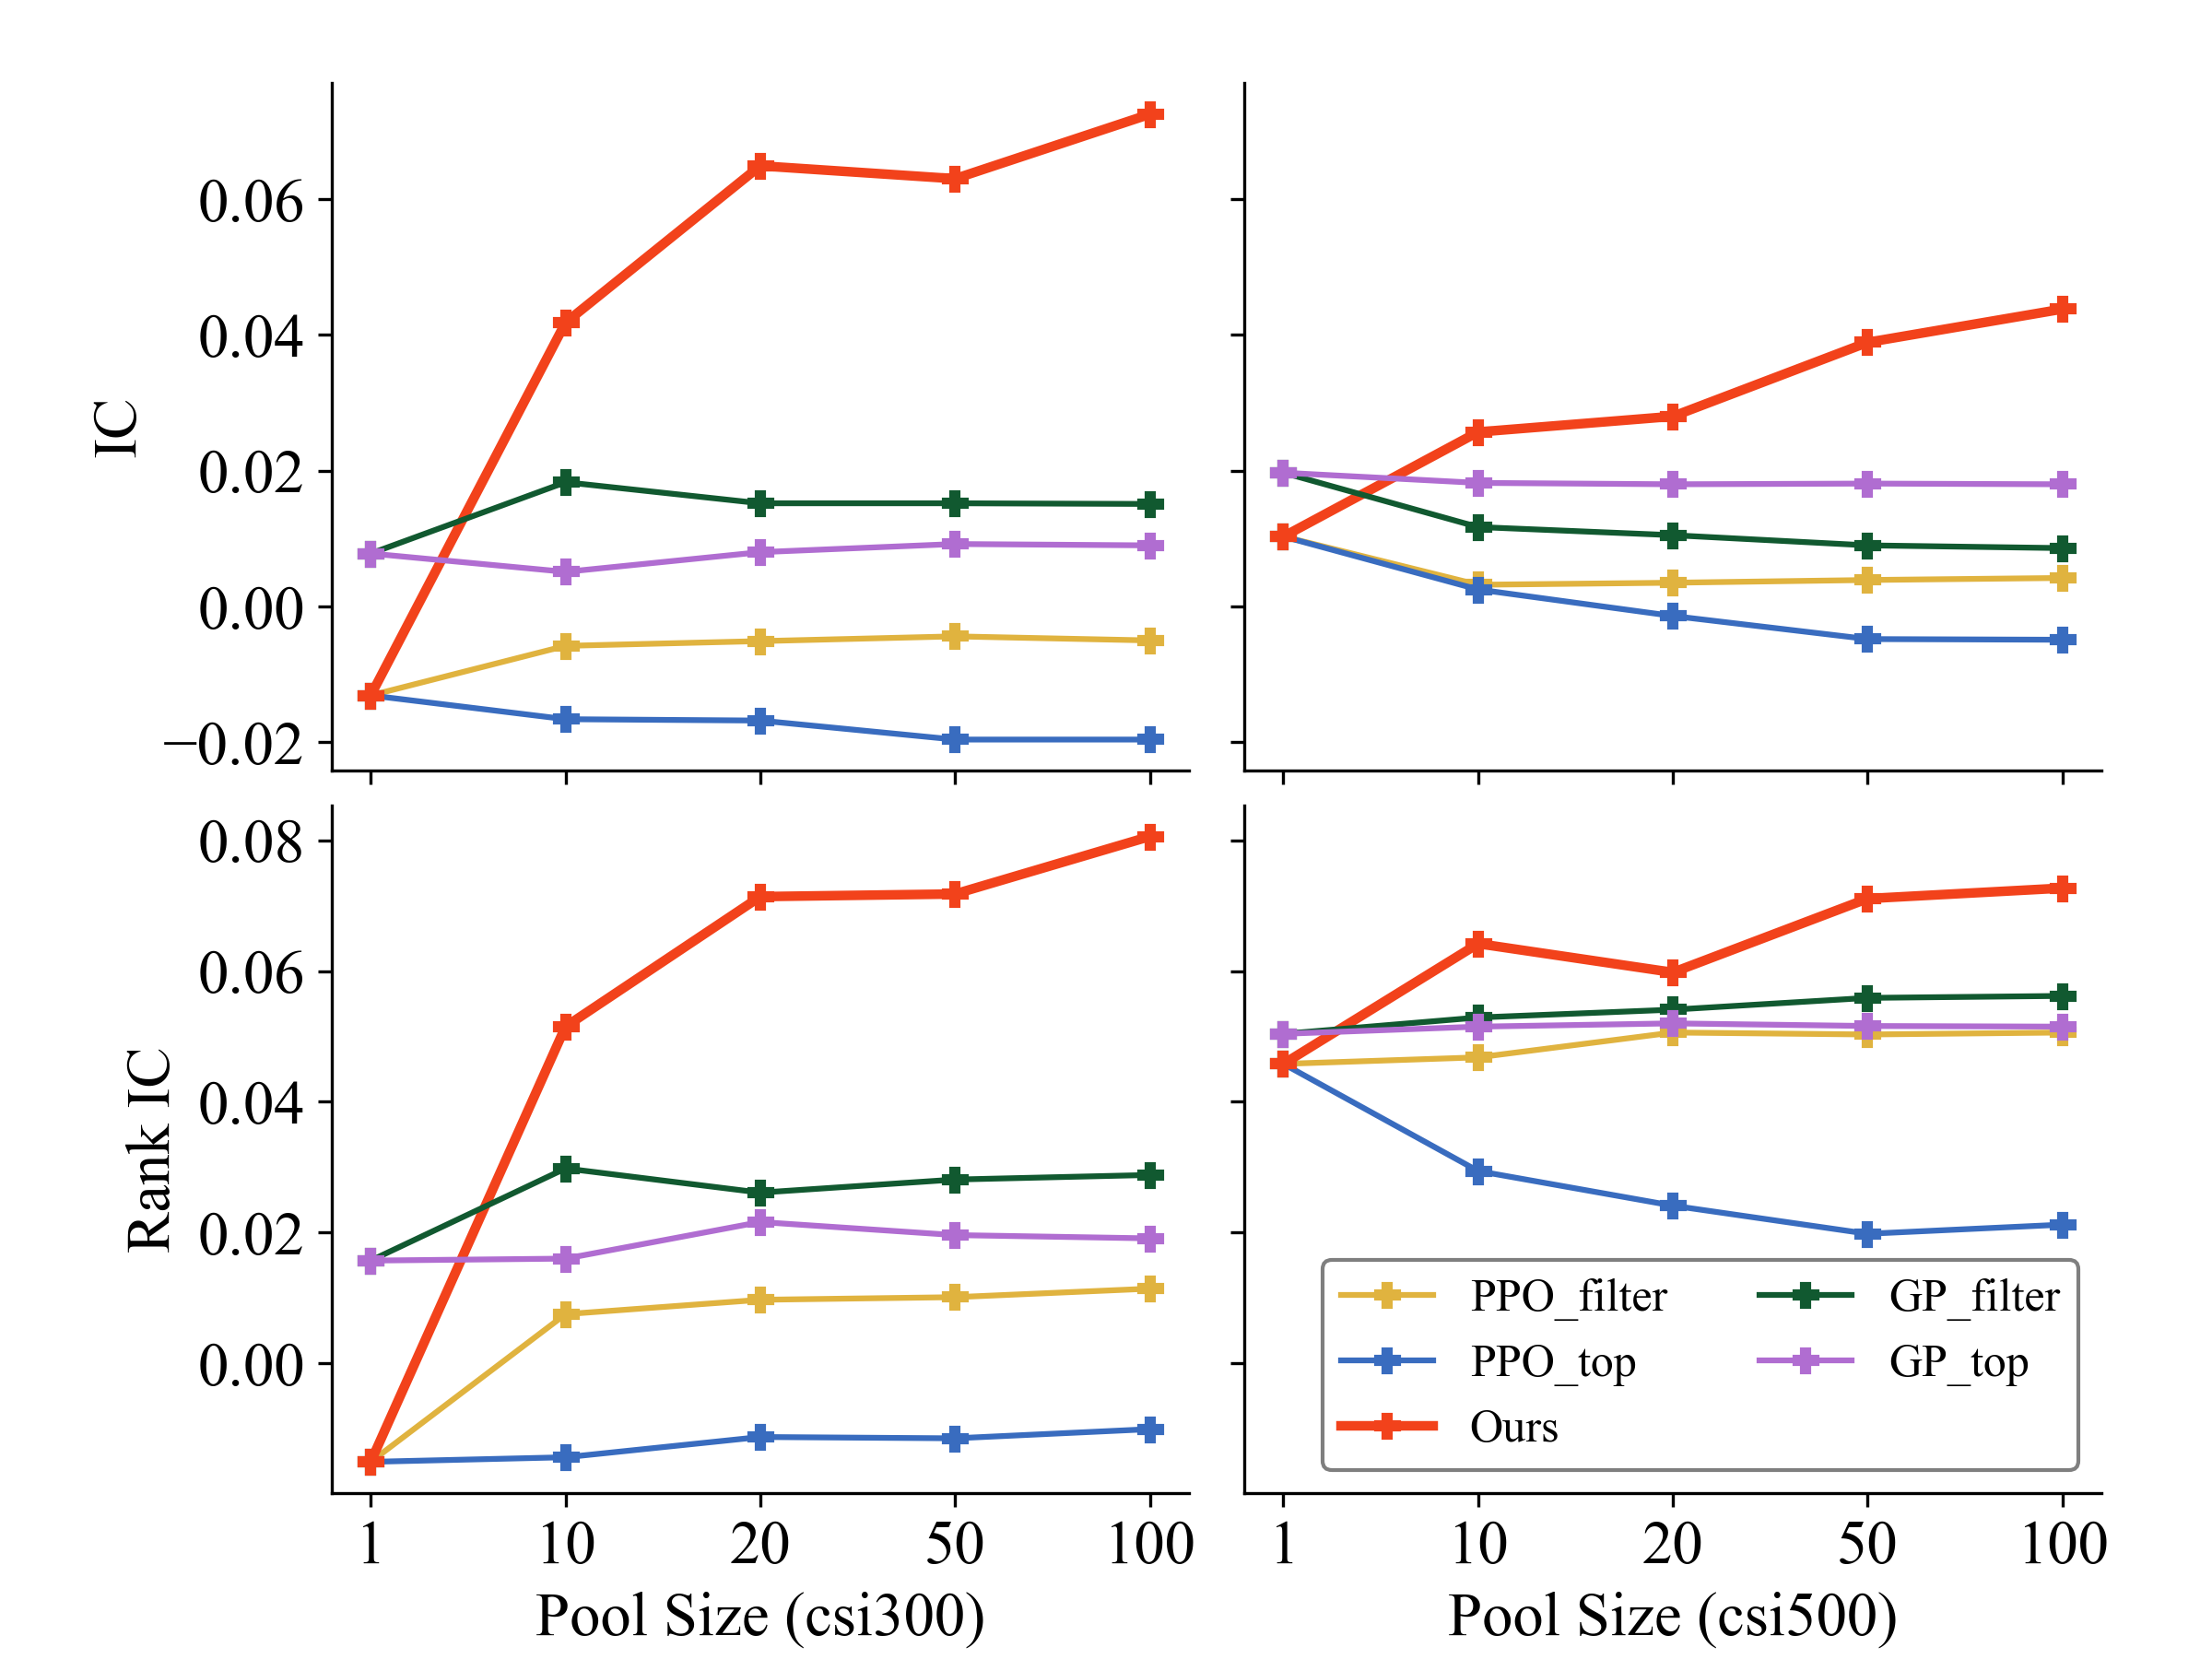
\includegraphics[width=1.08\linewidth]{Images/ablation.png}}
    \caption{The results of ablation study. A pool size of 1 refers to settings that only evaluate the top-most alpha without using a combination model.}
    \label{fig:ablation}
\end{figure}

\begin{table*}[ht]
    \centering
    \caption{An example combination of 10 alphas.}
    %\resizebox{0.96\textwidth}{!}{
    \begin{tabular}{>{\centering\arraybackslash}p{0.03\textwidth} | >{\centering\arraybackslash}p{0.6\textwidth} | >{\centering\arraybackslash}p{0.14\textwidth} >{\centering\arraybackslash}p{0.14\textwidth}}
        \toprule[1.5pt]
        \# & Alpha & Weight & IC (CSI300) \\
        \midrule[1pt] 1 & $\mathrm{Var}(\mathrm{Greater}(\mathrm{Greater}(\mathrm{Var}(\mathrm{low},50),\mathrm{high}),\mathrm{open}),30)$
        & $-0.0295$ & \cellcolor{p0000}$\hphantom{-}0.0011$ \\
        2 & $\mathrm{Max}((\mathrm{Min}(\mathrm{Max}(\mathrm{close}, 20) - 30, 20) + 100) / 30, 20)$
        & $\hphantom{-}0.0515$ & \cellcolor{p0025}$\hphantom{-}0.0262$ \\
        3 & $(\mathrm{Mad}(\mathrm{high}, 50) + 0.5)\mathrm{vwap} / \mathrm{close}$
        & $\hphantom{-}0.0343$ & \cellcolor{p0040}$\hphantom{-}0.0447$ \\
        4 & $\mathrm{Ref}(\mathrm{low}, 50)$
        & $\hphantom{-}0.0260$ & \cellcolor{p0020}$\hphantom{-}0.0241$ \\
        5 & $\mathrm{Min}(\mathrm{high} / \mathrm{close}, 50) - \mathrm{Greater}(-0.05 / \mathrm{close}, -10)$
        & $\hphantom{-}0.0437$ & \cellcolor{n0025}$-0.0211$ \\
        6 & $\mathrm{Delta}(\mathrm{high}, 20) + \mathrm{high} - 12$
        & $-0.0997$ & \cellcolor{p0015}$\hphantom{-}0.0165$ \\
        7 & $\mathrm{Less}(\mathrm{Min}(2(\mathrm{vwap} - \mathrm{volume}), 30) + 30, 30 \mathrm{vwap} / \mathrm{low}) - 5$
        & $\hphantom{-}0.0276$ & \cellcolor{p0000}$\hphantom{-}0.0025$ \\
        8 & $\mathrm{Corr}(\mathrm{Greater}(\mathrm{Greater}(\mathrm{vwap}, \mathrm{volume}),\mathrm{Greater}(\mathrm{close},$ \newline $\mathrm{Greater}(\mathrm{Log}(\mathrm{Var}(\mathrm{volume},10)),10))/\mathrm{close}),\mathrm{close},10)$
        & $-0.0279$ & \cellcolor{n0035}$-0.0338$ \\
        9 & $|\mathrm{low} - 30|$
        & $\hphantom{-}0.0319$ & \cellcolor{p0005}$\hphantom{-}0.0073$ \\
        10 & $\mathrm{Max}(1 - \mathrm{Max}(\mathrm{Corr}(\mathrm{low}, \mathrm{volume} \cdot \mathrm{Log}(10^{-4}\mathrm{Max}(\mathrm{volume}, 10)), 10), 10), 30)$
        & $\hphantom{-}0.0312$ & \cellcolor{p0045}$\hphantom{-}0.0488$ \\
        \hline
        \multicolumn{3}{c}{Weighted Combination} & \cellcolor{p0050}$\hphantom{-}0.0511$ \\
        \bottomrule[1.5pt]
    \end{tabular}%}
    \label{tab:case_study}
\end{table*}

\subsection{Main Results}

\subsubsection{Comparison across all alpha generators}

To answer \textbf{Q1}, we first compare our framework against several other alpha-mining methods and direct stock trend forecasting baselines, including PPO, GP, MLP, LightGBM, and XGBoost. Experiments are conducted on CSI300 and CSI500 stocks respectively.

The results are shown in Table \ref{tab:main_ic_rankic}. Our framework is able to achieve the highest IC and rank IC across all the methods we compare to. Note that the framework is only explicitly optimized against the IC metric. The non-formulaic alpha models come in the second tier. The baseline formulaic alpha generators perform poorly on the test set, especially the RL-based ones. The reinforcement learning agent, when optimized only against single-alpha IC, is prone to falling into local optima and thus overfitting on the training set, and basically stops searching for new alphas after a certain amount of steps. On the other hand, the GP-based methods maintaining a large population can avoid the same problem, but still cannot produce alphas that are synergistic when used together. The results also show that the filtering techniques cannot solve the synergy problem consistently either.

\subsubsection{Comparison of formulaic generators with varying pool capacity} \label{sec:ablation}

To answer \textbf{Q2}, we study the four baseline formulaic alpha generators more extensively, and compare them to our proposed framework. The models are evaluated under pool sizes of $k \in \braces{1, 10, 20, 50, 100}$. The results are shown in Figure \ref{fig:ablation}.

Compared to the baseline method PPO\_filter, our method directly uses the combination model's performance as the reward to newly generated alphas. This leads to a substantial improvement when the pool size increases, meaning that our method can produce alpha sets with great synergy. Our method shows scalability for pool size: even when the pool size is large enough, it can still continuously find synergistic alphas that boost the performance over the existing pool. Conversely, the combined performance of the alphas generated by other approaches barely improves upon the case with just the top alpha, meaning that these alpha factors have poor synergy. Furthermore, the ability to control the reward of individual expressions under a certain alpha pool configuration is granted by the flexibility of the RL scheme. The GP scheme of maintaining a large population at the same time does not work well with fine-grained fitness value control.

Also, we can see that for the CSI500 dataset, GP\_filter performs worse than GP\_top on the IC metric when the pool size increases. This phenomenon demonstrates that the traditionally used mutual-IC filtering is not always effective, answering the question \textbf{Q3}.

\subsection{Case Study}

Table \ref{tab:case_study} shows an example combination of 10 alphas generated by our framework, evaluated on the CSI300 constituent stock set. Most of the alpha pairs in this specific set have mutual IC values over 0.7. Previous work \cite{huataigp}\cite{autoalpha} considered this to be too high for the individual alphas to be regarded as ``diverse'', yet these alphas are able to work well in a synergistic manner. For example, the alphas \#2 and \#6 have a mutual IC of $0.9746$, thus traditionally considered too similar to be useful cooperatively. However, the combination $0.09317f_2 - 0.07163f_6$ achieves an IC of $0.0458$ on the test set, even higher than the sum of the respective ICs, showing the synergy effect.

Also, although alpha \#1 only has an IC of 0.0011, it still plays a vital role in the final combination. Once we remove alpha \#1 from the combination and re-train the combination weights on the remaining set, the combination's IC drops to merely $0.0447$. The two observations above show that neither the single alpha IC nor the mutual IC between alpha pairs is a good indicator of how well the combined alpha would perform, answering \textbf{Q3}.

One possible explanation for these phenomena is that: Although traditionally these alphas are similar due to the high mutual IC, some linear combinations of the alphas could point to a completely different direction from the original ones. Consider two unit vectors in a linear space. The more similar these two vectors are, the less similar either of these vectors is to the difference between the two vectors, since the difference vector approaches to be perpendicular to either of the original vectors as the vectors get closer.\

\begin{figure*}[]
    \centering
    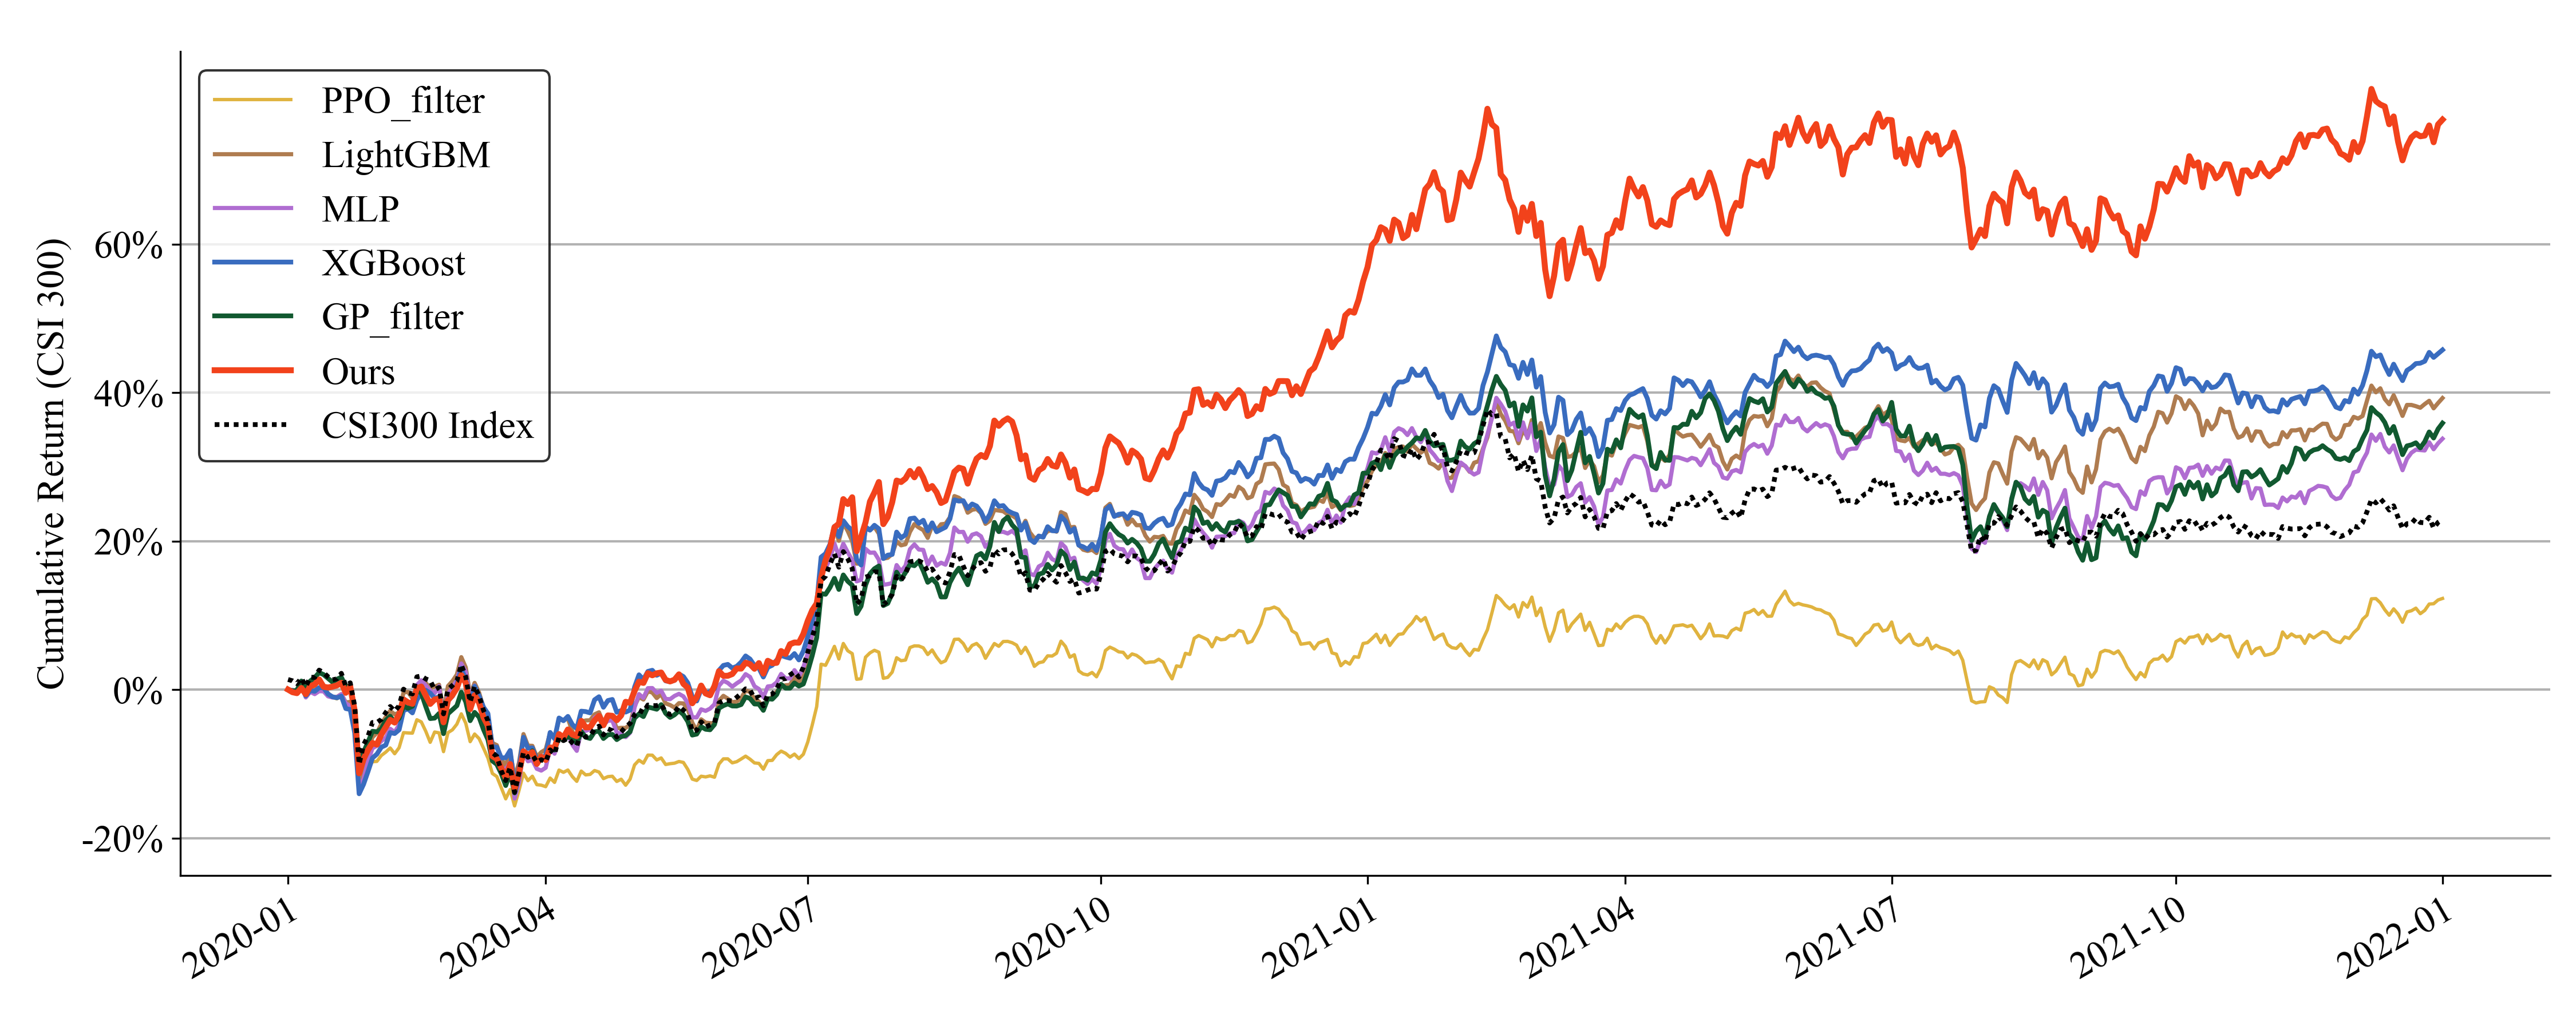
\includegraphics[width=1.0\linewidth]{Images/backtest.png}
    \caption{Backtest results on CSI 300. The lines track the net worth of simulated trading agents utilizing the various alpha-mining approaches.}
    \label{fig:backtest}
\end{figure*}

\subsection{Investment Simulation}

To demonstrate the effectiveness of our factors in more realistic investing settings, we use a simple investment strategy and conducted backtests in the testing period (2020/01/01 to 2021/12/31) on the CSI300 dataset. We use a simple \emph{top-$k$/drop-$n$} strategy to simulate the investment: On each trading day, we first sort the alpha values of the stocks, and then select the top $k$ stocks in that sorted list. We evenly invest across the $k$ stocks if possible, but restrict the strategy to only buy/sell at most $n$ stocks on each day to reduce excessive trading costs. In our experiment, $k$ is set to 50 and $n$ to 5.

We recorded the net worth of the respective strategies in the testing period, of which a line chart is shown in Figure \ref{fig:backtest}. Although our framework does not explicitly optimize towards the absolute returns, the framework still performs well in the backtest. Our framework is able to gain the most profit compared to the other methods.
